% Options for packages loaded elsewhere
\PassOptionsToPackage{unicode}{hyperref}
\PassOptionsToPackage{hyphens}{url}
%
\documentclass[
  ,jou,floatsintext]{apa6}
\usepackage{amsmath,amssymb}
\usepackage{lmodern}
\usepackage{iftex}
\ifPDFTeX
  \usepackage[T1]{fontenc}
  \usepackage[utf8]{inputenc}
  \usepackage{textcomp} % provide euro and other symbols
\else % if luatex or xetex
  \usepackage{unicode-math}
  \defaultfontfeatures{Scale=MatchLowercase}
  \defaultfontfeatures[\rmfamily]{Ligatures=TeX,Scale=1}
\fi
% Use upquote if available, for straight quotes in verbatim environments
\IfFileExists{upquote.sty}{\usepackage{upquote}}{}
\IfFileExists{microtype.sty}{% use microtype if available
  \usepackage[]{microtype}
  \UseMicrotypeSet[protrusion]{basicmath} % disable protrusion for tt fonts
}{}
\makeatletter
\@ifundefined{KOMAClassName}{% if non-KOMA class
  \IfFileExists{parskip.sty}{%
    \usepackage{parskip}
  }{% else
    \setlength{\parindent}{0pt}
    \setlength{\parskip}{6pt plus 2pt minus 1pt}}
}{% if KOMA class
  \KOMAoptions{parskip=half}}
\makeatother
\usepackage{xcolor}
\usepackage{graphicx}
\makeatletter
\def\maxwidth{\ifdim\Gin@nat@width>\linewidth\linewidth\else\Gin@nat@width\fi}
\def\maxheight{\ifdim\Gin@nat@height>\textheight\textheight\else\Gin@nat@height\fi}
\makeatother
% Scale images if necessary, so that they will not overflow the page
% margins by default, and it is still possible to overwrite the defaults
% using explicit options in \includegraphics[width, height, ...]{}
\setkeys{Gin}{width=\maxwidth,height=\maxheight,keepaspectratio}
% Set default figure placement to htbp
\makeatletter
\def\fps@figure{htbp}
\makeatother
\setlength{\emergencystretch}{3em} % prevent overfull lines
\providecommand{\tightlist}{%
  \setlength{\itemsep}{0pt}\setlength{\parskip}{0pt}}
\setcounter{secnumdepth}{-\maxdimen} % remove section numbering
% Make \paragraph and \subparagraph free-standing
\ifx\paragraph\undefined\else
  \let\oldparagraph\paragraph
  \renewcommand{\paragraph}[1]{\oldparagraph{#1}\mbox{}}
\fi
\ifx\subparagraph\undefined\else
  \let\oldsubparagraph\subparagraph
  \renewcommand{\subparagraph}[1]{\oldsubparagraph{#1}\mbox{}}
\fi
\newlength{\cslhangindent}
\setlength{\cslhangindent}{1.5em}
\newlength{\csllabelwidth}
\setlength{\csllabelwidth}{3em}
\newlength{\cslentryspacingunit} % times entry-spacing
\setlength{\cslentryspacingunit}{\parskip}
\newenvironment{CSLReferences}[2] % #1 hanging-ident, #2 entry spacing
 {% don't indent paragraphs
  \setlength{\parindent}{0pt}
  % turn on hanging indent if param 1 is 1
  \ifodd #1
  \let\oldpar\par
  \def\par{\hangindent=\cslhangindent\oldpar}
  \fi
  % set entry spacing
  \setlength{\parskip}{#2\cslentryspacingunit}
 }%
 {}
\usepackage{calc}
\newcommand{\CSLBlock}[1]{#1\hfill\break}
\newcommand{\CSLLeftMargin}[1]{\parbox[t]{\csllabelwidth}{#1}}
\newcommand{\CSLRightInline}[1]{\parbox[t]{\linewidth - \csllabelwidth}{#1}\break}
\newcommand{\CSLIndent}[1]{\hspace{\cslhangindent}#1}
\ifLuaTeX
\usepackage[bidi=basic]{babel}
\else
\usepackage[bidi=default]{babel}
\fi
\babelprovide[main,import]{english}
% get rid of language-specific shorthands (see #6817):
\let\LanguageShortHands\languageshorthands
\def\languageshorthands#1{}
% Manuscript styling
\usepackage{upgreek}
\captionsetup{font=singlespacing,justification=justified}

% Table formatting
\usepackage{longtable}
\usepackage{lscape}
% \usepackage[counterclockwise]{rotating}   % Landscape page setup for large tables
\usepackage{multirow}		% Table styling
\usepackage{tabularx}		% Control Column width
\usepackage[flushleft]{threeparttable}	% Allows for three part tables with a specified notes section
\usepackage{threeparttablex}            % Lets threeparttable work with longtable

% Create new environments so endfloat can handle them
% \newenvironment{ltable}
%   {\begin{landscape}\centering\begin{threeparttable}}
%   {\end{threeparttable}\end{landscape}}
\newenvironment{lltable}{\begin{landscape}\centering\begin{ThreePartTable}}{\end{ThreePartTable}\end{landscape}}

% Enables adjusting longtable caption width to table width
% Solution found at http://golatex.de/longtable-mit-caption-so-breit-wie-die-tabelle-t15767.html
\makeatletter
\newcommand\LastLTentrywidth{1em}
\newlength\longtablewidth
\setlength{\longtablewidth}{1in}
\newcommand{\getlongtablewidth}{\begingroup \ifcsname LT@\roman{LT@tables}\endcsname \global\longtablewidth=0pt \renewcommand{\LT@entry}[2]{\global\advance\longtablewidth by ##2\relax\gdef\LastLTentrywidth{##2}}\@nameuse{LT@\roman{LT@tables}} \fi \endgroup}

% \setlength{\parindent}{0.5in}
% \setlength{\parskip}{0pt plus 0pt minus 0pt}

% Overwrite redefinition of paragraph and subparagraph by the default LaTeX template
% See https://github.com/crsh/papaja/issues/292
\makeatletter
\renewcommand{\paragraph}{\@startsection{paragraph}{4}{\parindent}%
  {0\baselineskip \@plus 0.2ex \@minus 0.2ex}%
  {-1em}%
  {\normalfont\normalsize\bfseries\itshape\typesectitle}}

\renewcommand{\subparagraph}[1]{\@startsection{subparagraph}{5}{1em}%
  {0\baselineskip \@plus 0.2ex \@minus 0.2ex}%
  {-\z@\relax}%
  {\normalfont\normalsize\itshape\hspace{\parindent}{#1}\textit{\addperi}}{\relax}}
\makeatother

% \usepackage{etoolbox}
\makeatletter
\patchcmd{\HyOrg@maketitle}
  {\section{\normalfont\normalsize\abstractname}}
  {\section*{\normalfont\normalsize\abstractname}}
  {}{\typeout{Failed to patch abstract.}}
\patchcmd{\HyOrg@maketitle}
  {\section{\protect\normalfont{\@title}}}
  {\section*{\protect\normalfont{\@title}}}
  {}{\typeout{Failed to patch title.}}
\makeatother

\usepackage{xpatch}
\makeatletter
\xapptocmd\appendix
  {\xapptocmd\section
    {\addcontentsline{toc}{section}{\appendixname\ifoneappendix\else~\theappendix\fi\\: #1}}
    {}{\InnerPatchFailed}%
  }
{}{\PatchFailed}
\usepackage{dblfloatfix}


\usepackage{csquotes}
\ifLuaTeX
  \usepackage{selnolig}  % disable illegal ligatures
\fi
\IfFileExists{bookmark.sty}{\usepackage{bookmark}}{\usepackage{hyperref}}
\IfFileExists{xurl.sty}{\usepackage{xurl}}{} % add URL line breaks if available
\urlstyle{same} % disable monospaced font for URLs
\hypersetup{
  pdftitle={Faith in Reason: developing a survey measure of belief in the rationality of others},
  pdfauthor={Tom Stafford1, Junyan Zhu2, \& Katharine Dommett2},
  pdflang={en-EN},
  hidelinks,
  pdfcreator={LaTeX via pandoc}}

\title{Faith in Reason: developing a survey measure of belief in the rationality of others}
\author{Tom Stafford\textsuperscript{1}, Junyan Zhu\textsuperscript{2}, \& Katharine Dommett\textsuperscript{2}}
\date{}


\shorttitle{Faith in Reason}

\authornote{

For the purpose of open access, the author has applied a Creative Commons Attribution (CC BY) licence to any Author Accepted Manuscript version arising.

Document prepared with RMarkdown (Allaire et al., 2020) and papaja (Aust \& Barth, 2020). CRediT (Contributor Roles Taxonomy) autogenerated using Tenzing (Holcombe, Kovacs, Aust, \& Aczel, 2020). Template is available here \href{https://github.com/tomstafford/rmarkdown_apa}{github.com/tomstafford/rmarkdown\_apa}

The authors made the following contributions. Tom Stafford: Conceptualization, Data curation, Formal analysis, Funding acquisition, Methodology, Visualization, Writing - original draft, Writing - review \& editing; Junyan Zhu: Conceptualization, Data curation, Formal analysis, Methodology, Visualization, Writing - original draft, Writing - review \& editing; Katharine Dommett: Conceptualization, Funding acquisition, Methodology, Writing - review \& editing.

Correspondence concerning this article should be addressed to Tom Stafford, Department of Psychology, University of Sheffield, Sheffield, UK. E-mail: \href{mailto:t.stafford@sheffield.ac.uk}{\nolinkurl{t.stafford@sheffield.ac.uk}}

}

\affiliation{\vspace{0.5cm}\textsuperscript{1} Department of Psychology, University of Sheffield, UK\\\textsuperscript{2} Department of Politics and International Relations, University of Sheffield, UK}

\note{\textcolor{red}{Preprint 2023-04-21}}

\abstract{%
abstract goes here
}



\begin{document}
\maketitle

\hypertarget{introduction}{%
\section{Introduction}\label{introduction}}

What we believe about other people matters. It is not enough that others \emph{are} trustworthy, reasonable or well intentioned. Successful coordination, as well as individual wellbeing, benefit when we also \emph{perceive} others as trustworthy, reasonable or well intentioned.

\hypertarget{rationality}{%
\subsection{Rationality}\label{rationality}}

The nature of human reason is a perennial topic. Human rationality has been praised (``a thinking reed'') and condemned (``TK'') by different thinkers. The so-called `Rationality Wars' (TK) centered around the definition of rationality that might reasonably used as a standard against which to judge human reasoning

An influential research programme is the heuristics and biases programme in psychology (TK), which uses the ideal of economic rationality as a standard to define actual human reasoning against. From this perspective human reasoning appears riddled with biases, but much work is done by the adoption of the standards of utility theory, formal logic and precise statistical reasoning.

Mercier and Sperber's argumentative theory of reasons provides an account TK
TK cite my Frontiers paper, BBC commentary

\hypertarget{criteria-of-reason}{%
\subsection{Criteria of reason}\label{criteria-of-reason}}

So rationality is not a unitary concept, nor one around which there is consensus on the definition of, despite the way it is often evoked in discussion (and particularly in discussion of its negation e.g.~``they are being irrational'').

That said, core features of rationality have been proposed.

Dawson, N. V., \& Gregory, F. (2009). Correspondence and coherence in science: A brief historical perspective. Judgment and decision making, 4(2), 126-133.

\hypertarget{insight}{%
\subsubsection{Insight}\label{insight}}

Nisbett, R. E., \& Wilson, T. D. (1977). Telling more than we can know: Verbal reports on mental processes. Psychological review, 84(3), 231.

\hypertarget{influence-gullibility}{%
\subsubsection{Influence / Gullibility}\label{influence-gullibility}}

Altay, S., \& Acerbi, A. (2023). People believe misinformation is a threat because they assume others are gullible. New Media \& Society, 0(0). \url{https://doi.org/10.1177/14614448231153379}

Confidence in their abilities, friends' and family's abilities, and people's abilities to spot misinformation was measured with three statements adapted from Corbu et al.~(2020) and the European Commission (2018):
``I am able to identify news or information that misrepresent reality or is even false''
``My friends and family are able to identify news or information that misrepresent reality or is even false''
``People in general are able to identify news or information that misrepresent reality or is even false''

\begin{itemize}
\tightlist
\item
  negatively conceived
\item
  unidimensional: influence
\end{itemize}

Summary: so core features of rationality include coherance, correspondence, surceptibility to influence and insight into causes of ones actions. The extent to which these features form a coherent whole in the minds of the general public, and can meaningfully be asked about questions about is the primary topic of this paper.

\hypertarget{consequence-of-a-lack-of-faith-in-reason}{%
\subsection{Consequence of a lack of faith in reason}\label{consequence-of-a-lack-of-faith-in-reason}}

\hypertarget{second-order-effexcts-of-disinfo}{%
\subsubsection{Second order effexcts of Disinfo}\label{second-order-effexcts-of-disinfo}}

The generalised belief that others are well informed and reasonable is foundational to democracy. Recent concerns around misinformation may have second order effects, undermining democracy not by generating a misinformed populace, but by generating a populace that believes others are misunformed or unreasonable (Karpf, 2019). Alarmism around misinformation may potentially lower trust in institutions (Hoes, Clemm von Hohenberg, Gessler, Wojcieszak, \& Qian, 2022), increase skepticism about democracy (Jungherr \& Rauchfleisch, 2022; Nisbet, Mortenson, \& Li, 2021), or foster calls of tighter media regulation (Lee, 2021).

\hypertarget{third-person-effect}{%
\subsubsection{Third person effect}\label{third-person-effect}}

There is an established literature of the perception of media influence on others (Perloff, 2002; Sun, Pan, \& Shen, 2008). The `third person effect', proposed by Davison (1983), is the phenomenon whereby many people believe others are more susceptible to influence than themselves. The third person effect was proposed as a root cause of censorship instincts and this has been confirmed by subsequent empricial investigations (Feng \& Guo, 2012; Olshansky \& Landrum, 2020).

Two caveats around the third person effect. Lyons (2022) has recently argued that - for many people - a third person effect of greater media influence on others rather than the self will be an accurate perception. Chung and Moon (2016) have argued that the driving factor in many so-called third person effects is the perception of others (as highly influenced), rather than the discrepancy with first person perception per se.

TK we directly measured the TPE!!

\hypertarget{generalised-trust}{%
\subsection{Generalised trust}\label{generalised-trust}}

social capital, dropped wallets, democracy

\hypertarget{method}{%
\section{Method}\label{method}}

Part of a larger survey

\hypertarget{sample}{%
\subsection{Sample}\label{sample}}

\hypertarget{item-development}{%
\subsection{Item development}\label{item-development}}

correspondance (items 2 and 6)
coherance (items 7 and 8)
influence (items 3 and 5)
insight into behaviour (4)
naive endorsement (item 1)

See Table \ref{tab:items}

\begin{table*}[tbp]

\begin{center}
\begin{threeparttable}

\caption{\label{tab:items}Scale item wording}

\begin{tabular}{ll}
\toprule
nums & \multicolumn{1}{c}{items}\\
\midrule
1 & The typical person is often irrational\\
2 & People are often misinformed on important issues\\
3 & People are too easily manipulated\\
4 & People often act for reasons they don’t understand or endorse\\
5 & The average person can be persuaded to change their mind if given good reasons\\
6 & Most people hold accurate views about the world\\
A & For this question please click the middle option, ‘neutral’, to show you are paying attention\\
7 & An individual's beliefs about the world are generally coherent\\
8 & People's behaviour is generally consistent with their beliefs\\
\bottomrule
\addlinespace
\end{tabular}

\begin{tablenotes}[para]
\normalsize{\textit{Note.} Response was on a 7 point Likert scale from (1 = "Strong Disagree", 7 = "Strongly Agree"). Items 1,2,3 and 4 reverse coded so that for all items higher scores represented stronger faith in reason.}
\end{tablenotes}

\end{threeparttable}
\end{center}

\end{table*}

\hypertarget{prereg}{%
\subsection{Prereg}\label{prereg}}

\hypertarget{reproducibility}{%
\subsection{Reproducibility}\label{reproducibility}}

Data availability: The analysis code and anonymised response data which support the results here are openly available \url{https://github.com/tomstafford/faithinreason}

This repository contains the files used to generate this report, which is in the form of a \texttt{reproducible\ manuscript}, a document which generates the analysis it reports, and so combines sharing, documenting and reporting an analysis in a single set of project files.

\hypertarget{results}{%
\section{Results}\label{results}}

\hypertarget{initial-characterisations}{%
\subsection{Initial characterisations}\label{initial-characterisations}}

Our data consist of 1875 participants who completed our online survey. 6 failed an attention check and were removed.

\begin{figure}

{\centering 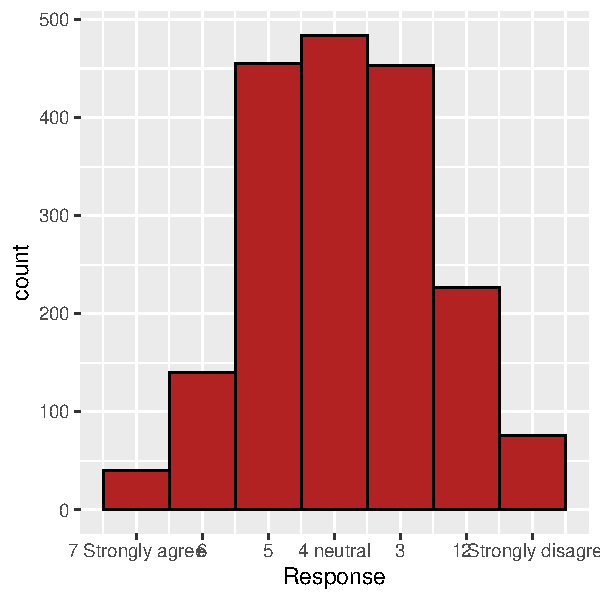
\includegraphics[width=0.75\linewidth]{faithinreason_files/figure-latex/ourhistogram-1} 

}

\caption{Histogram of responses to Item 1 ("The typical person is often irrational")}\label{fig:ourhistogram}
\end{figure}

\hypertarget{scale-development-item-selection}{%
\subsection{scale development / item selection}\label{scale-development-item-selection}}

\begin{figure}

{\centering 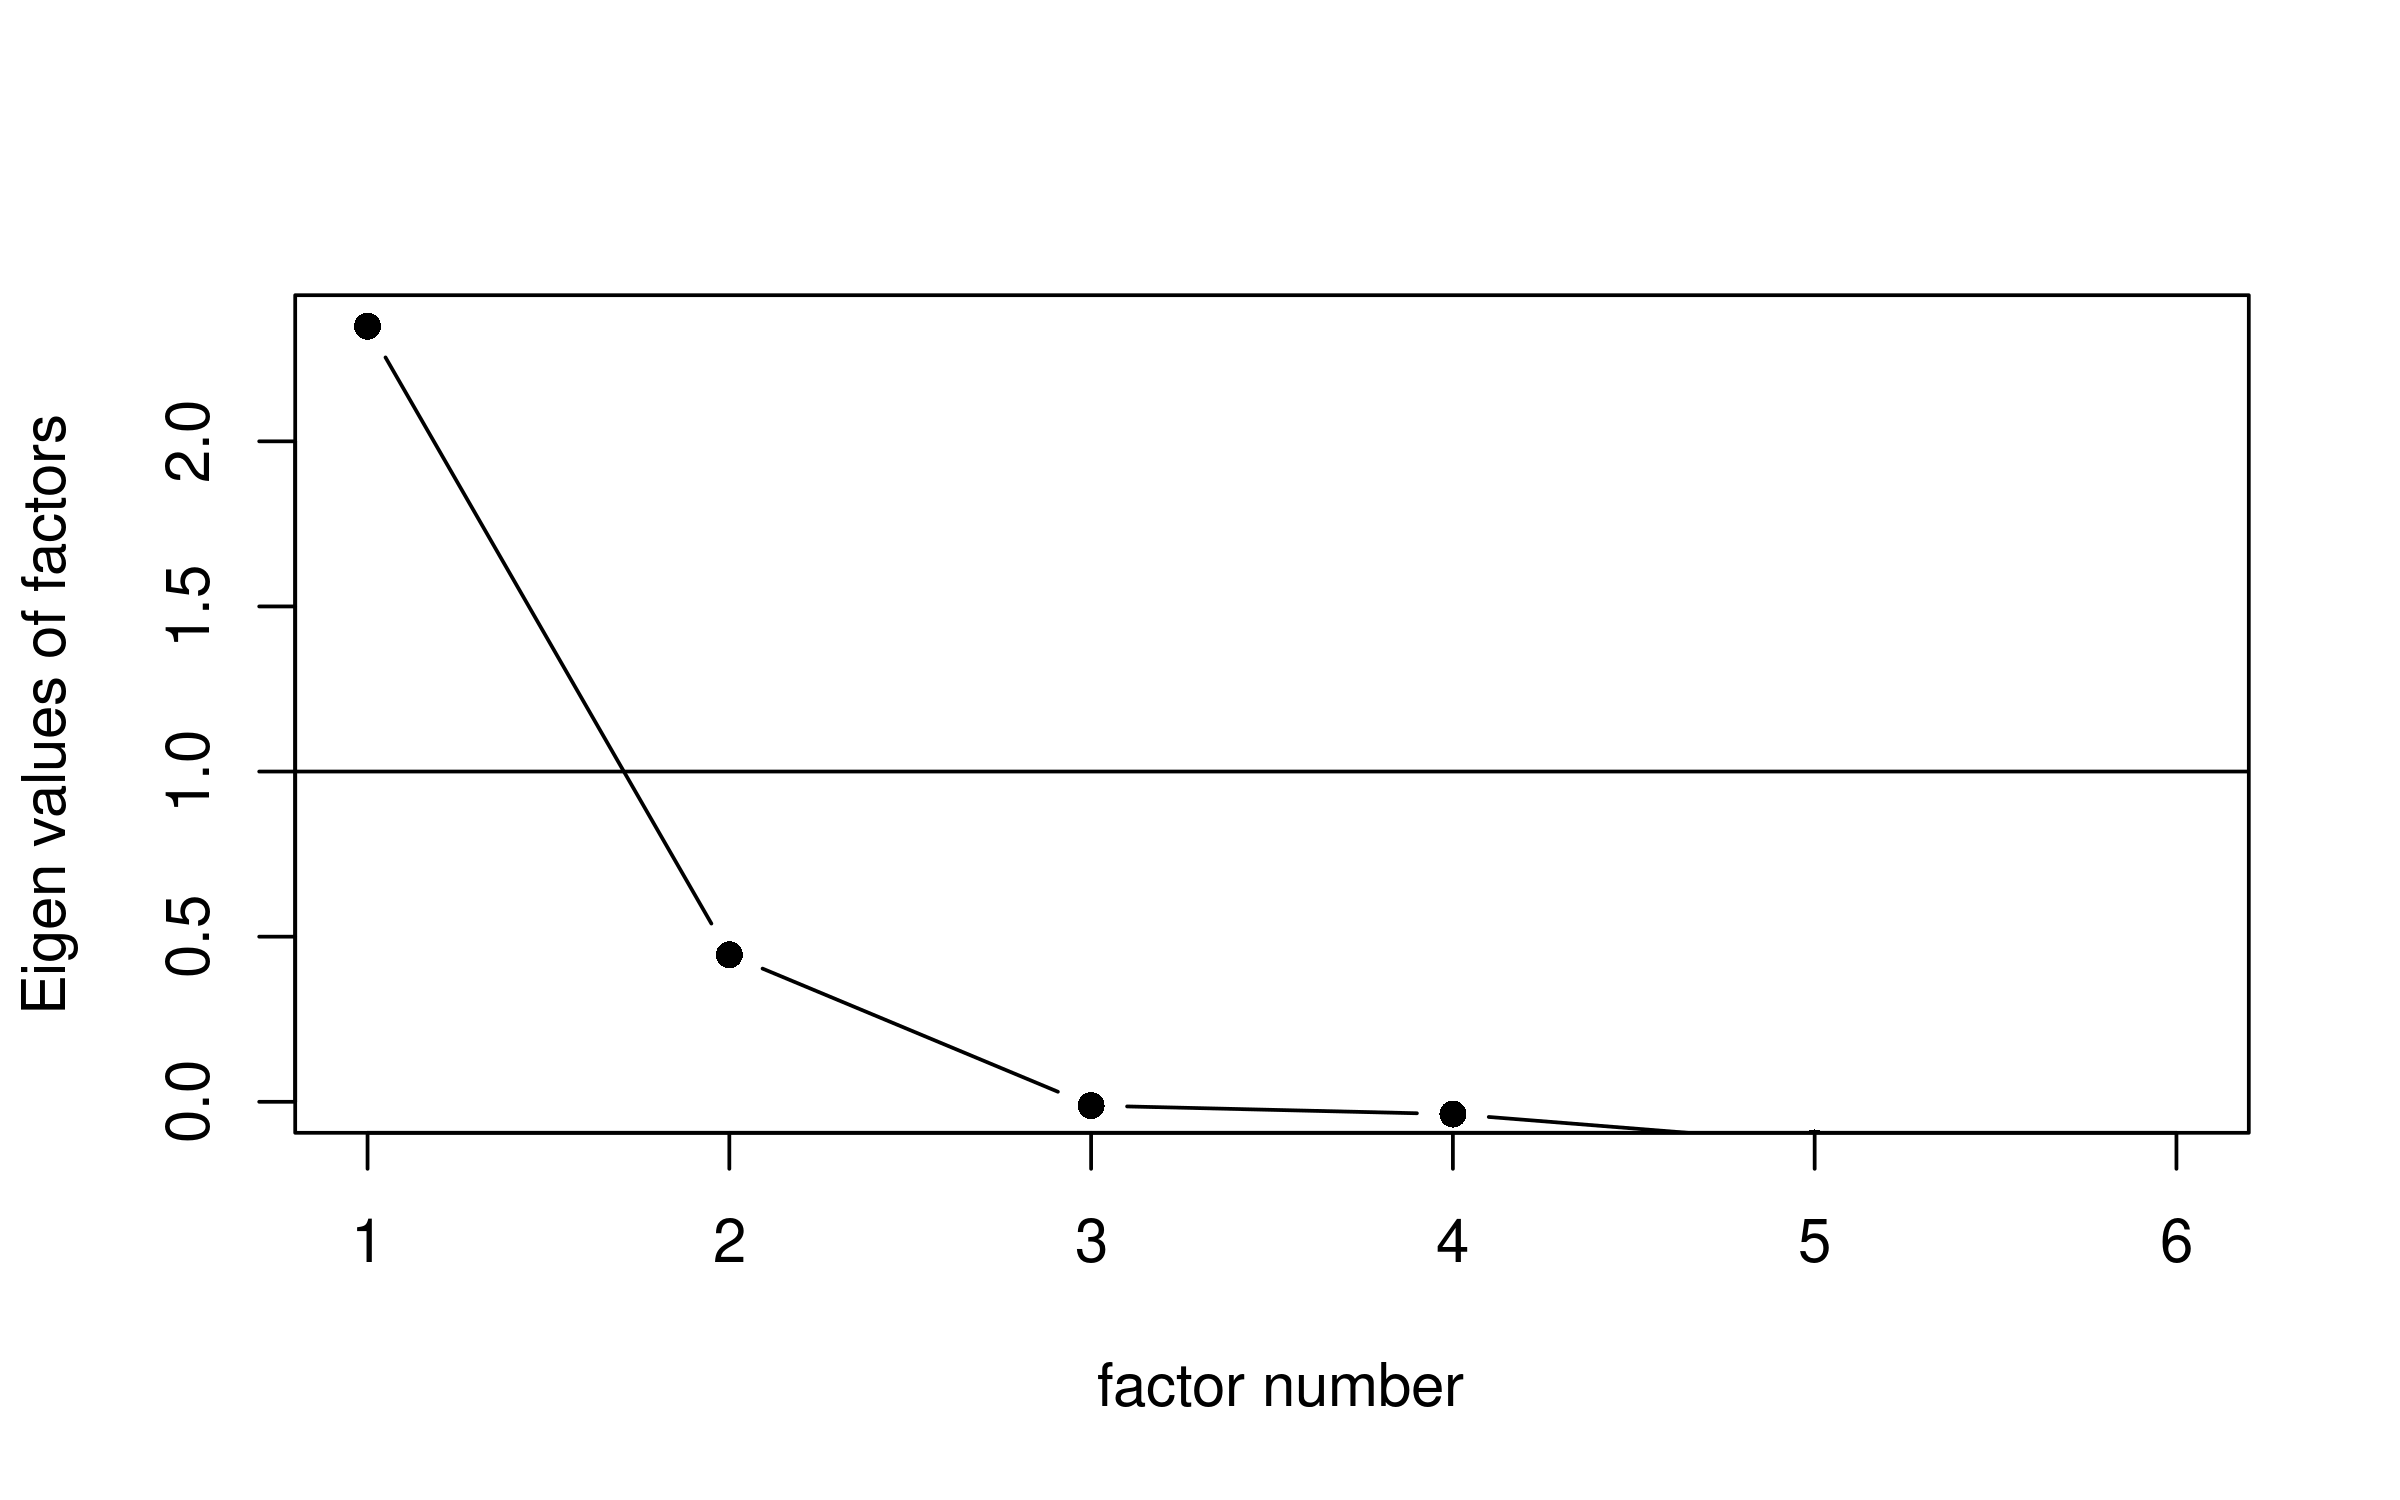
\includegraphics[width=1\linewidth]{plots/reason_scree6} 

}

\caption{Factor analysis}\label{fig:factors}
\end{figure}

\begin{figure}

{\centering 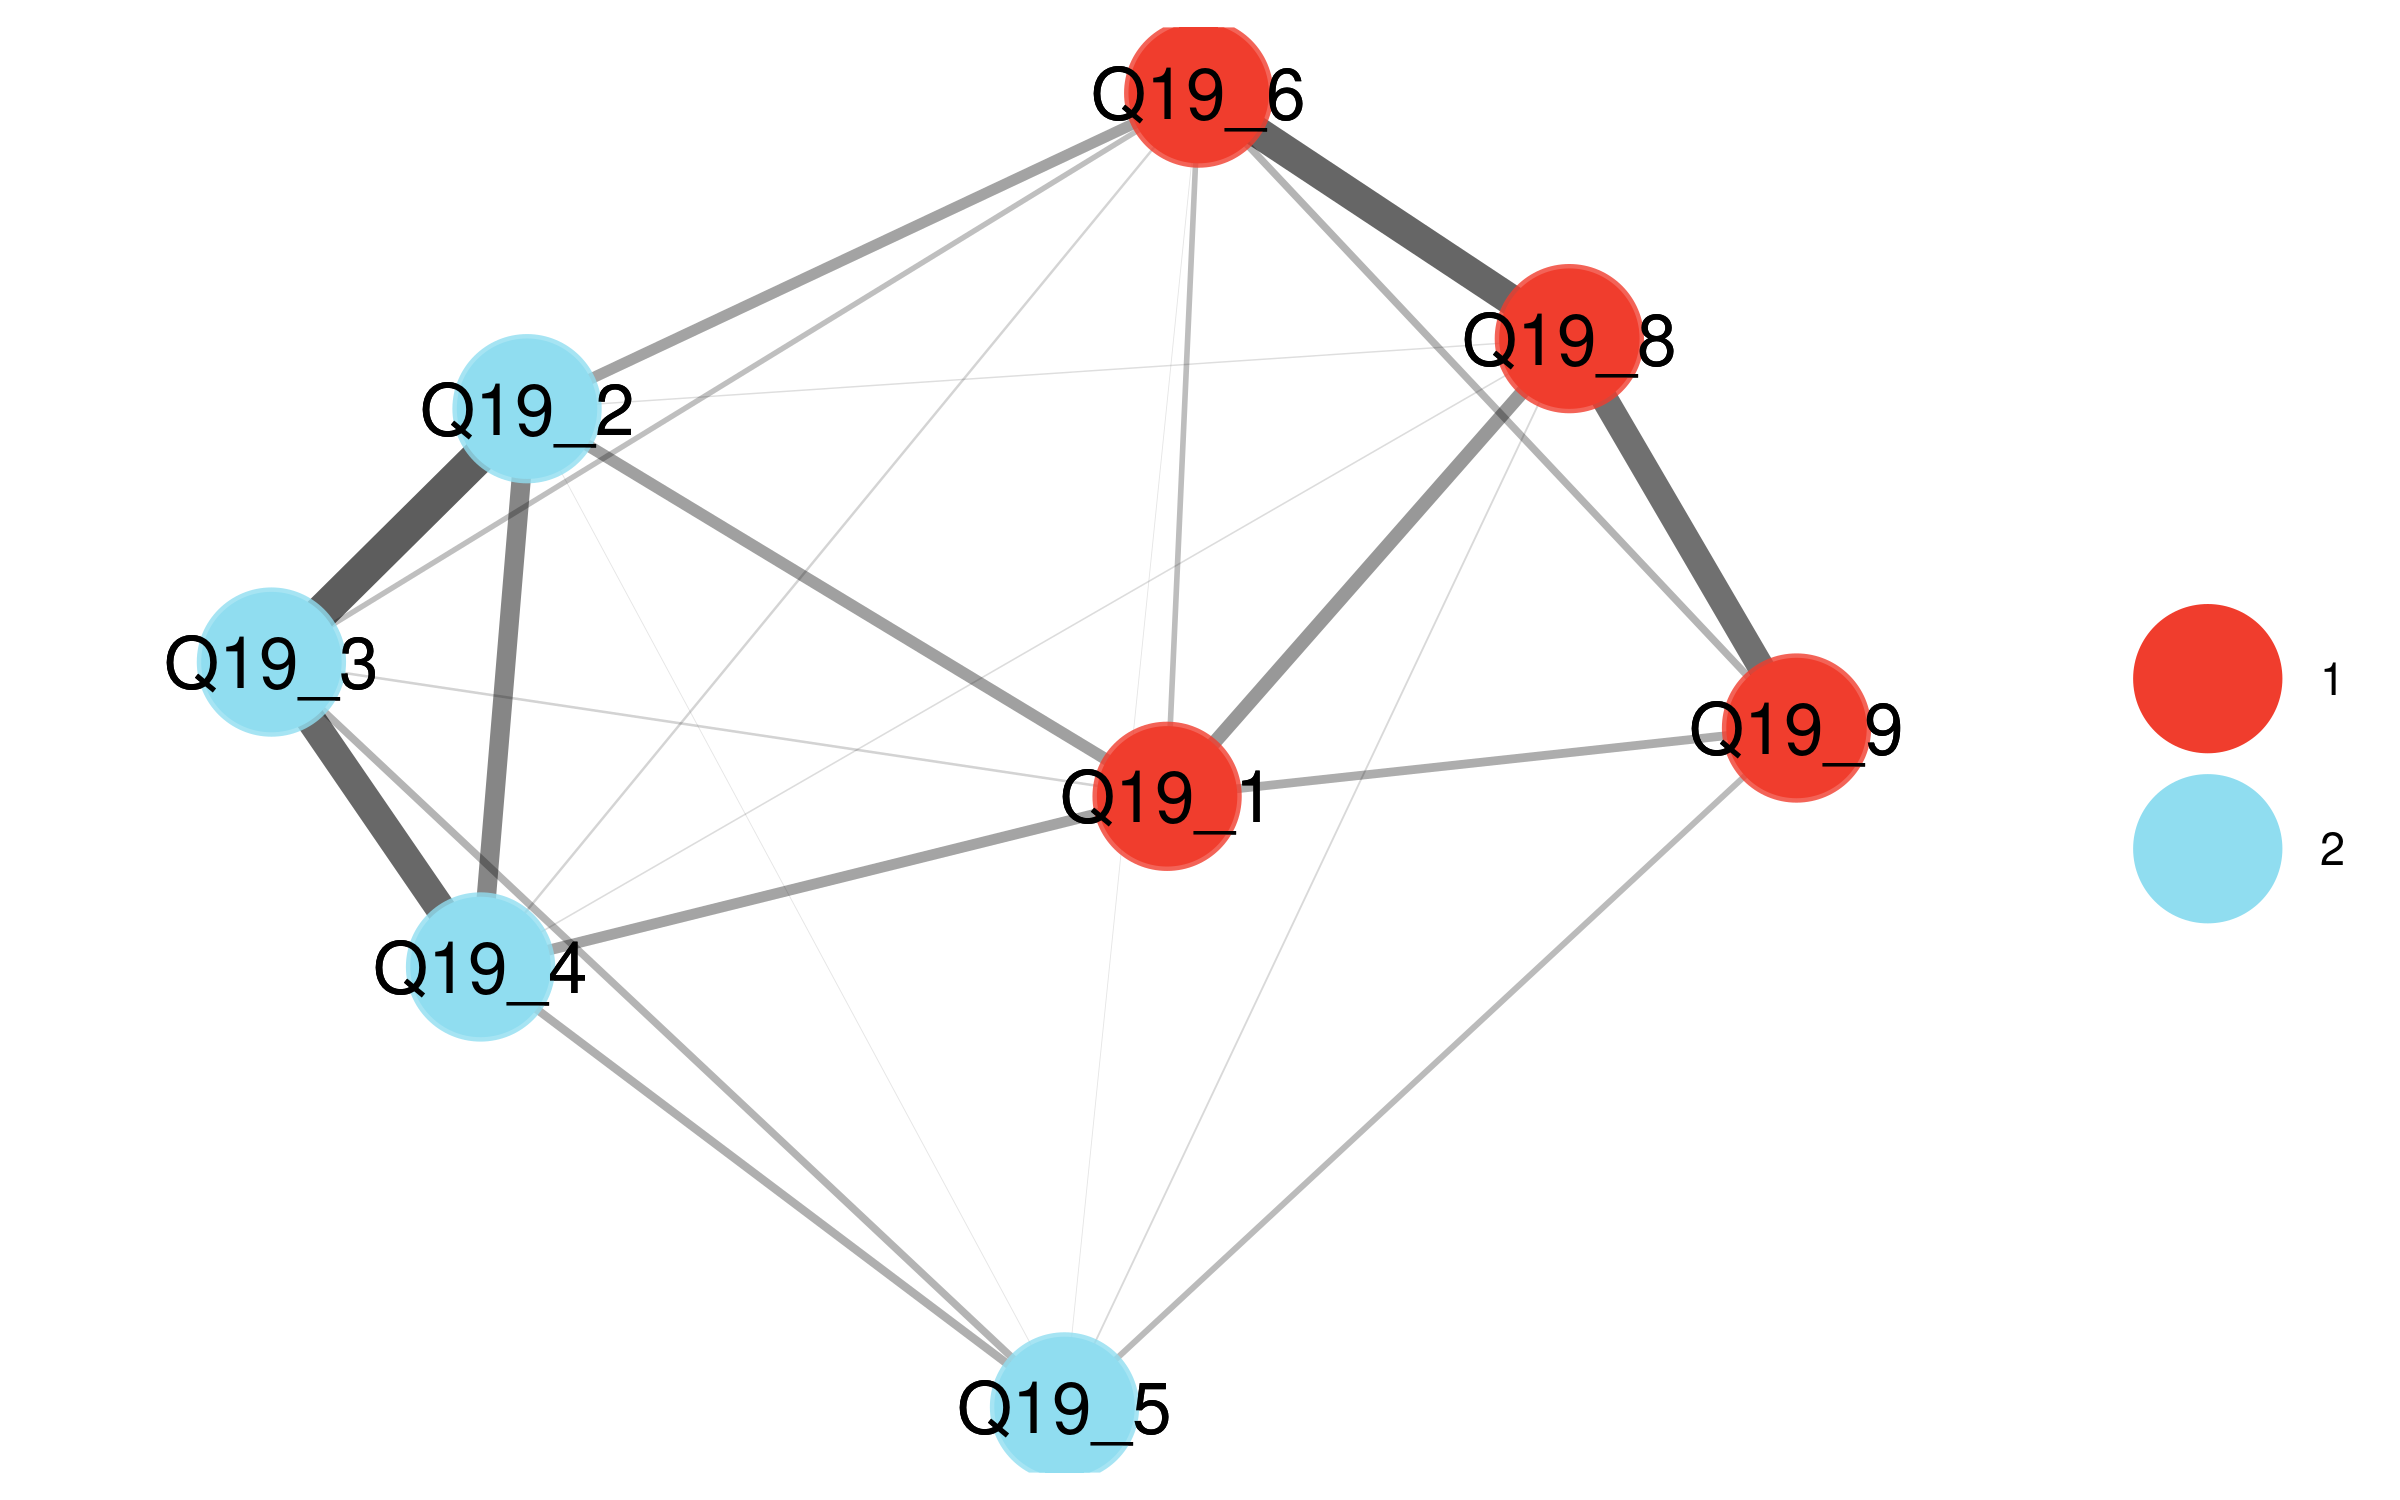
\includegraphics[width=1\linewidth]{plots/reason_ega} 

}

\caption{Exploratory Graph Analysis (EGA) of all items.}\label{fig:egafull}
\end{figure}

\begin{figure}

{\centering 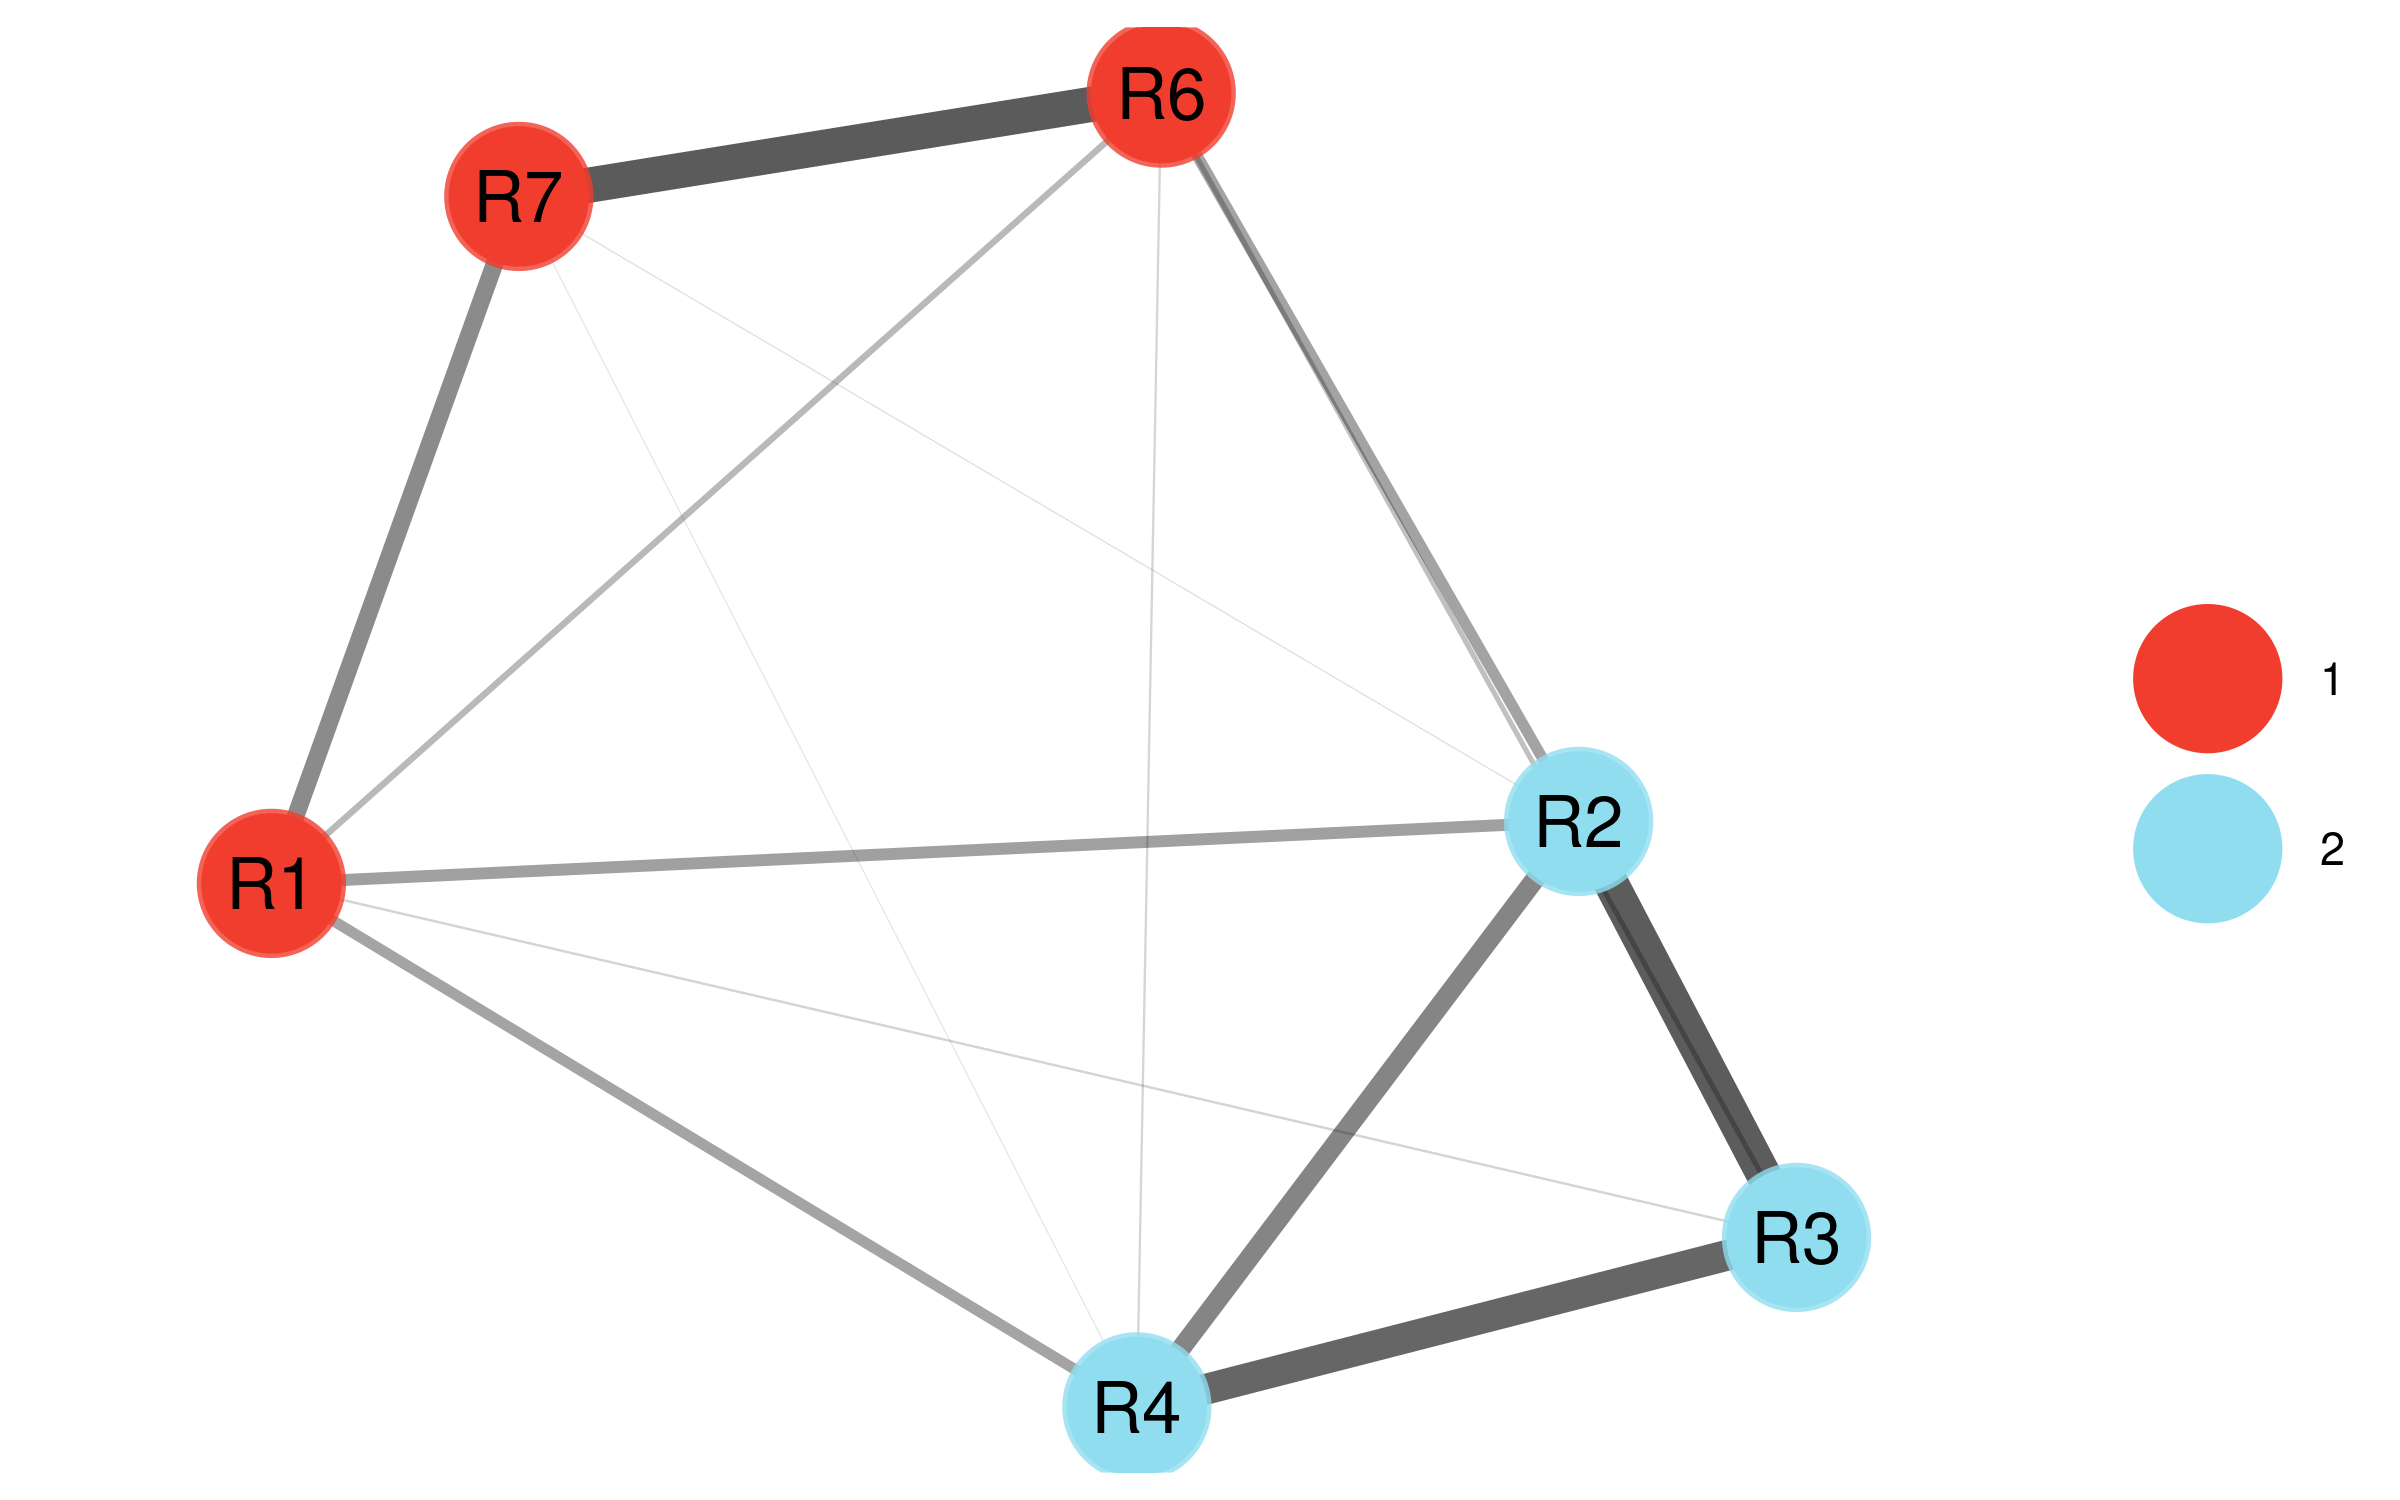
\includegraphics[width=1\linewidth]{plots/reason6_ega} 

}

\caption{The items of the full ASRS scale displayed following Exploratory Graph Analysis (EGA).}\label{fig:egasix}
\end{figure}

\hypertarget{scale-analysis}{%
\subsection{Scale analysis}\label{scale-analysis}}

\begin{figure}

{\centering 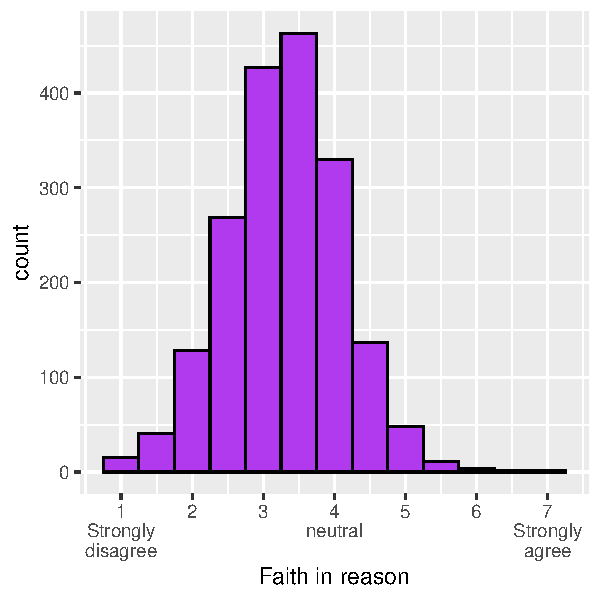
\includegraphics[width=0.75\linewidth]{faithinreason_files/figure-latex/meanhistogram-1} 

}

\caption{Histogram of mean of responses to all rationality items}\label{fig:meanhistogram}
\end{figure}

The average score across these six items was 3.29, a summary statistic which suggests that the typical view of other people weighted to being slightly less, rather than slightly more, reasonable. The distribution is shown in Figure \ref{fig:meanhistogram}.

\begin{figure}

{\centering 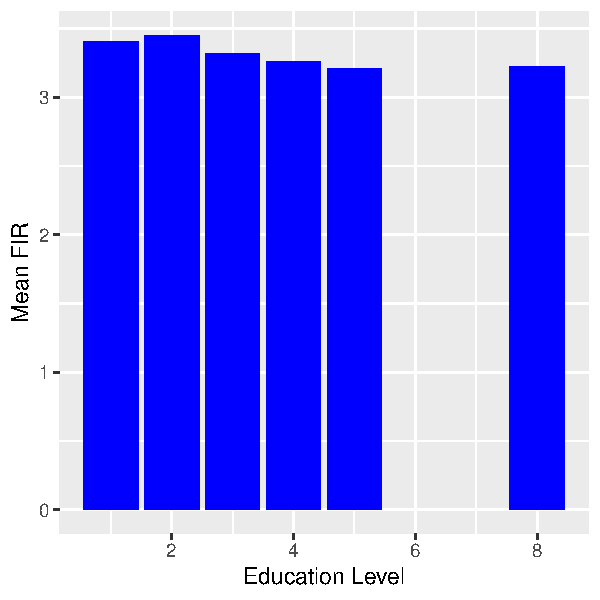
\includegraphics[width=0.75\linewidth]{faithinreason_files/figure-latex/education-1} 

}

\caption{Education level and mean FIR}\label{fig:education}
\end{figure}
\begin{figure}

{\centering 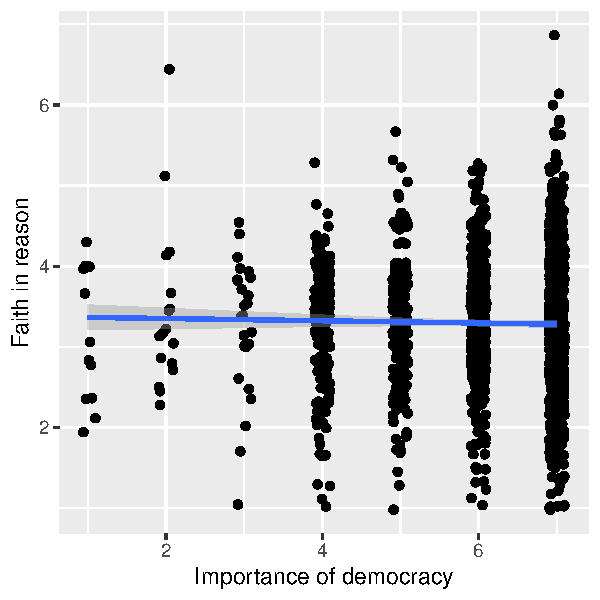
\includegraphics[width=0.75\linewidth]{faithinreason_files/figure-latex/democract-1} 

}

\caption{How important is it for you to live in a country that is governed democratically? and mean FIR}\label{fig:democract}
\end{figure}

\begin{figure}

{\centering 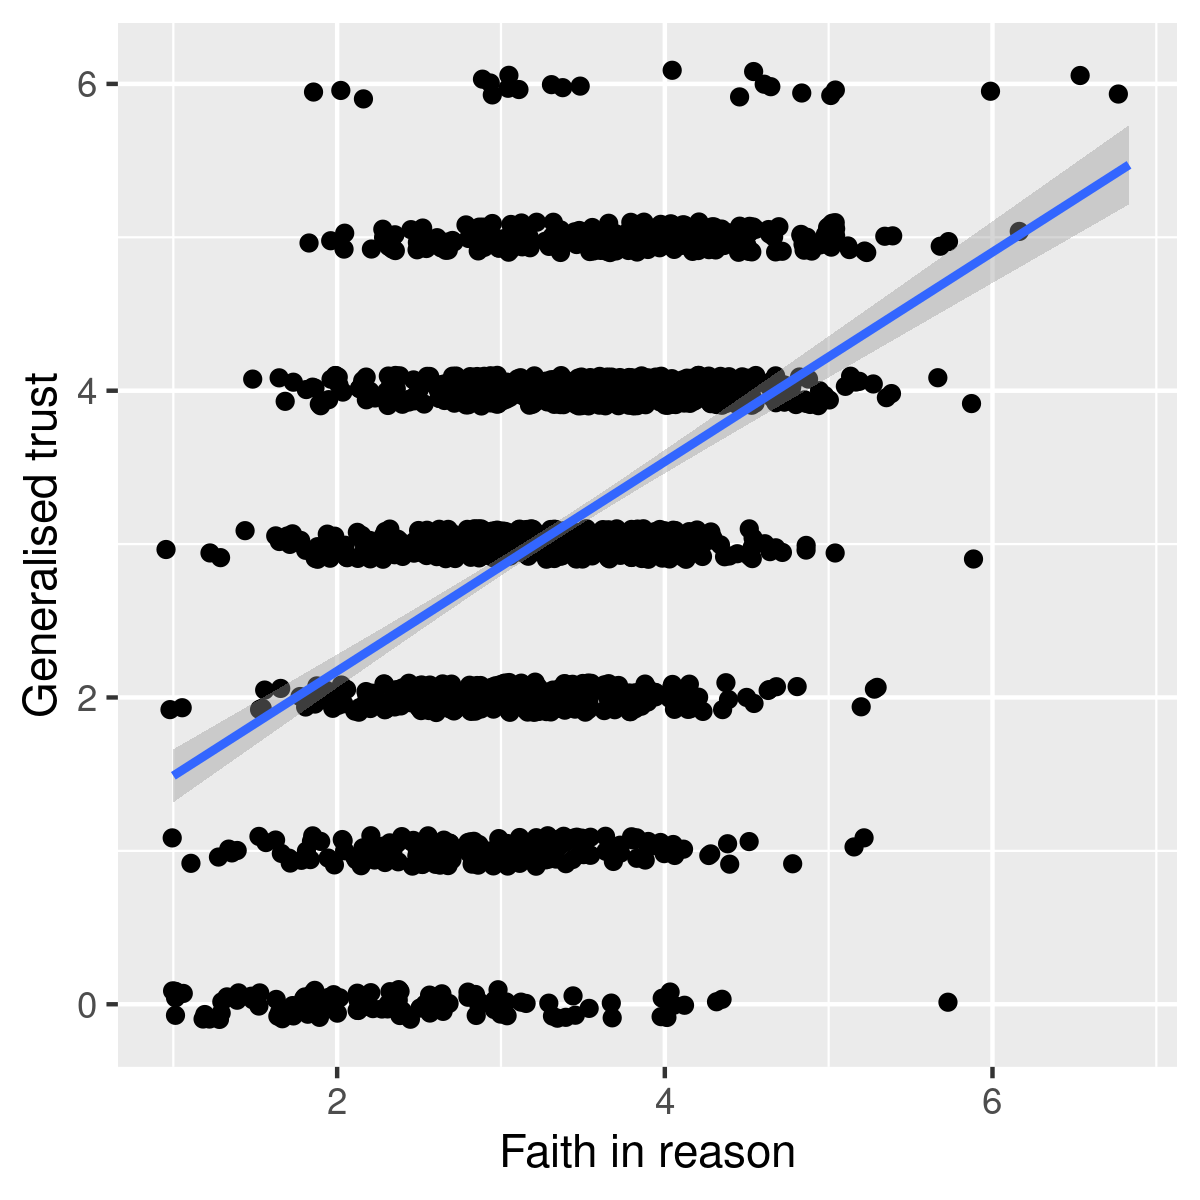
\includegraphics[width=0.75\linewidth]{faithinreason_files/figure-latex/generalisetrust-1} 

}

\caption{Generally speaking, would you say that most people can be trusted? and mean FIR}\label{fig:generalisetrust}
\end{figure}

Correlation between Q17 and FIR

\begin{table}

\caption{\label{tab:correlations}Correlation Matrix}
\centering
\begin{tabular}[t]{l|r|r|r}
\hline
  & mean & Q16 & Q17\\
\hline
mean & 1.00 & -0.02 & 0.40\\
\hline
Q16 & -0.02 & 1.00 & 0.26\\
\hline
Q17 & 0.40 & 0.26 & 1.00\\
\hline
\end{tabular}
\end{table}

\hypertarget{todo}{%
\subsection{TODO}\label{todo}}

Methods for assessing dimensionality
cronbach's alpha + leave on out
scree plots and EFA
Mokken scale analysis
EGA

Write up all of them?

Look at items and make sensible decisions. A single scale of 6 items and 2 subscales?

\hypertarget{junyan}{%
\subsection{Junyan}\label{junyan}}

We asked 8 questions about rationality in the survey. To determine the homogeneity and the
fitness of the responses, I use Stata to perform Mokken scaling analysis. Testing all 8
rationality variables, the Mokken analysis yields one scale of 6 items. The items with low
Loevinger's coefficient of homogeneity (H i ), a criterion for scalability, are dropped. If the
overall H\textless0.3, it means the items in the scale are unrelated, thus cannot be accepted to form a
cumulative scale. As a rule of thumb, H i must be higher than 0.3 to be kept in the scale.
Therefore, there are 6 fitting items in the scale: rationality\_1, rationality\_2, rationality\_3,
rationality\_4, rationality\_6, and rationality\_7. The overall H coefficient is 0.41, indicating a
medium-strong scalability. The individual critical values in the scale are all lower than 80, so
the variables are double monotonous and there is no model violation.
Code: loevh rationality\_1 rationality\_2 rationality\_3 rationality\_4 rationality\_6 rationality\_7,
pair monotonicity(*) ppp pmm nipmatrix(minvi(0.03) siglevel(0.01))
We can thus generate a rationality variable by aggregating those six variables. Cronbach's \(\alpha\)
is 0.78, indicating an acceptable internal consistency.

Based on the statistical results, it looks to me that rationality\_5 (The average person can be
persuaded to change if given good reasons) is a real problem, it doesn't fit at all with other items

3
and must be removed. Rationality\_8 (People\textquotesingle s behaviour is generally consistent with their beliefs)
has a poor fitness, but it is not as bad as rationality\_5.

Next, I try to scale the remaining two items that are not included in the above scale --
rationality\_5 and rationality\_8. As expected, these two items doesn't form a separate scale.
Empirically, these items are excluded from the rationality measure by Mokken scaling likely
because persuasion effect is not a robust indication of rationality?

\hypertarget{tom}{%
\subsection{Tom}\label{tom}}

Obviously 5 is weakly correlated. Omitting gives biggest boost to Cronbach's alpha, EEGnet suggests weakly related to all other items,

EEGnet suggets two commuities
Scree plot of factors suggests border of unidimension and bidimensional
mokken analysis suggests 1 domension, BUT if you remove items 5 and 9 you then find 2 dim3nsions at 0.35

\hypertarget{discussion}{%
\section{Discussion}\label{discussion}}

\hypertarget{normative-models}{%
\subsection{Normative models}\label{normative-models}}

arguably our scale doesn't touch on normative models of rationality as captured by T\&K. Bias, prejudice

Deflationary accounts of misinformation (Mercier, 2020; Nyhan, 2020)

\hypertarget{references}{%
\section*{References}\label{references}}
\addcontentsline{toc}{section}{References}

\hypertarget{refs}{}
\begin{CSLReferences}{1}{0}
\leavevmode\vadjust pre{\hypertarget{ref-rmarkdowncite}{}}%
Allaire, J., Xie, Y., McPherson, J., Luraschi, J., Ushey, K., Atkins, A., \ldots{} Iannone, R. (2020). \emph{Rmarkdown: Dynamic documents for r}. Retrieved from \url{https://github.com/rstudio/rmarkdown}

\leavevmode\vadjust pre{\hypertarget{ref-aust2020}{}}%
Aust, F., \& Barth, M. (2020). \emph{{papaja}: {Create} {APA} manuscripts with {R Markdown}}. Retrieved from \url{https://github.com/crsh/papaja}

\leavevmode\vadjust pre{\hypertarget{ref-chung2016}{}}%
Chung, S., \& Moon, S.-I. (2016). Is the third-person effect real? A critical examination of rationales, testing methods, and previous findings of the third-person effect on censorship attitudes. \emph{Human Communication Research}, \emph{42}(2), 312--337.

\leavevmode\vadjust pre{\hypertarget{ref-davison1983}{}}%
Davison, W. P. (1983). The third-person effect in communication. \emph{Public Opinion Quarterly}, \emph{47}(1), 1--15.

\leavevmode\vadjust pre{\hypertarget{ref-feng2012}{}}%
Feng, G. C., \& Guo, S. Z. (2012). Support for censorship: A multilevel meta-analysis of the third-person effect. \emph{Communication Reports}, \emph{25}(1), 40--50.

\leavevmode\vadjust pre{\hypertarget{ref-hoes2022}{}}%
Hoes, E., Clemm von Hohenberg, B., Gessler, T., Wojcieszak, M., \& Qian, S. (2022). \emph{The cure worse than the disease? How the media's attention to misinformation decreases trust}. PsyArXiv. \url{https://doi.org/10.31234/osf.io/4m92p}

\leavevmode\vadjust pre{\hypertarget{ref-holcombe2020documenting}{}}%
Holcombe, A. O., Kovacs, M., Aust, F., \& Aczel, B. (2020). Documenting contributions to scholarly articles using CRediT and tenzing. \emph{PLoS One}, \emph{15}(12), e0244611.

\leavevmode\vadjust pre{\hypertarget{ref-jungherr2022}{}}%
Jungherr, A., \& Rauchfleisch, A. (2022). \emph{Negative downstream effects of disinformation discourse: Evidence from the US}. SocArXiv.

\leavevmode\vadjust pre{\hypertarget{ref-karpf2019}{}}%
Karpf, D. (2019). On digital disinformation and democratic myths. Retrieved from \url{https://mediawell.ssrc.org/expert-reflections/on-digital-disinformation-and-democratic-myths/}

\leavevmode\vadjust pre{\hypertarget{ref-lee2021}{}}%
Lee, T. (2021). How people perceive influence of fake news and why it matters. \emph{Communication Quarterly}, \emph{69}(4), 431--453.

\leavevmode\vadjust pre{\hypertarget{ref-lyons2022}{}}%
Lyons, B. A. (2022). Why we should rethink the third-person effect: Disentangling bias and earned confidence using behavioral data. \emph{Journal of Communication}, \emph{72}(5), 565--577.

\leavevmode\vadjust pre{\hypertarget{ref-mercier2020}{}}%
Mercier, H. (2020). \emph{Not born yesterday}. Princeton: Princeton University Press.

\leavevmode\vadjust pre{\hypertarget{ref-nisbet2021}{}}%
Nisbet, E. C., Mortenson, C., \& Li, Q. (2021). The presumed influence of election misinformation on others reduces our own satisfaction with democracy. \emph{Harvard Kennedy School Misinformation Review}.

\leavevmode\vadjust pre{\hypertarget{ref-nyhan2020facts}{}}%
Nyhan, B. (2020). Facts and myths about misperceptions. \emph{Journal of Economic Perspectives}, \emph{34}(3), 220--236.

\leavevmode\vadjust pre{\hypertarget{ref-olshansky2020}{}}%
Olshansky, A., \& Landrum, A. R. (2020). Third-person perceptions and calls for censorship of flat earth videos on YouTube. \emph{Media and Communication}, \emph{8}(2), 387--400.

\leavevmode\vadjust pre{\hypertarget{ref-perloff2002}{}}%
Perloff, R. M. (2002). The third-person effect. In \emph{Media effects} (pp. 499--516). Routledge.

\leavevmode\vadjust pre{\hypertarget{ref-sun2008}{}}%
Sun, Y., Pan, Z., \& Shen, L. (2008). Understanding the third-person perception: Evidence from a meta-analysis. \emph{Journal of Communication}, \emph{58}(2), 280--300.

\end{CSLReferences}


\end{document}
